
% Group addresses by affiliation; use superscriptaddress for long
% author lists, or if there are many overlapping affiliations.
% For Phys. Rev. appearance, change preprint to twocolumn.
% Choose pra, prb, prc, prd, pre, prl, prstab, prstper, or rmp for journal
%  Add 'draft' option to mark overfull boxes with black boxes
%  Add 'showpacs' option to make PACS codes appear
%  Add 'showkeys' option to make keywords appear
\documentclass[aps,prd,reprint,superscriptaddress]{revtex4-1}
%\documentclass[aps,prl,preprint,superscriptaddress]{revtex4-1}
%\documentclass[aps,prl,reprint,groupedaddress]{revtex4-1}
%\usepackage{bm}
\usepackage{amsmath}
\usepackage{lineno}
\usepackage{graphicx}
%<<<<<<< HEAD
%\input{papers_packages_command._include_tex}


%\newcommand\refsec[1]{\S\ref{sec:#1}}
%\newcommand\refeq[1]{Eq.~(\ref{eqn:#1})}
%\input{papers_packages_command._include_tex}
\newcommand\refsec[1]{\S\ref{sec:#1}}
\newcommand\refeq[1]{Eq.~(\ref{eqn:#1})}
\newcommand{\refssec}[1]{section~\ref{subsec:#1}}
\newcommand{\reffig}[1]{Fig.~\ref{fig:#1}}
%\newcommand{\apj}{ApJ}
\newcommand{\physrep}{Physics Reports}
\newcommand{\aapr}{A\&A Rev.}
\newcommand{\apjl}{ApJL}
\newcommand{\apjs}{ApJS}
\newcommand{\aap}{A\&A}
\newcommand{\mnras}{MNRAS}
%\newcommand{\prd}{Phys. Rev. D}
\newcommand{\physrev}{Phys. Rev.}
\newcommand{\physrevlett}{Phys. Rev. Lett.}
\newcommand{\jcap}{{\em JCAP }}
\newcommand{\aj}{AJ }



%>>>>>>> 683231e77bc036bad411dd2244ca99280568d723
\bibliographystyle{apsrev4-1}

\begin{document}
\graphicspath{{images/}}

%Title of paper
\title{External priors for the next generation of CMB experiments.}

\author{Alessandro Manzotti}
\email{\href{mailto:manzotti.alessandro@gmail.com}{manzotti.alessandro@gmail.com}}
\affiliation{Department of Astronomy \& Astrophysics, University of Chicago, Chicago IL 60637}
\affiliation{Kavli Institute for Cosmological Physics, Enrico Fermi Institute, University of Chicago, Chicago, IL 60637}
\author{Scott Dodelson}

\affiliation{Department of Astronomy \& Astrophysics, University of Chicago, Chicago IL 60637}
\affiliation{Kavli Institute for Cosmological Physics, Enrico Fermi Institute, University of Chicago, Chicago, IL 60637}
\affiliation{Fermilab Center for Particle Astrophysics, Fermi National Accelerator Laboratory, Batavia, IL 60510-0500}

\date{\today}
\begin{abstract}
The next generation of cosmic microwave background (CMB) experiments can dramatically improve what we know about neutrino physics, inflation, Dark Matter and Dark Energy. 
Indeed the low level of noise, together with improved angular resolution, will drastically increase the signal to noise of the CMB polarized signal as well as the reconstructed lensing potential of high redshift large scale structure. 
Projected constraints on cosmological parameters are extremely tight, but these can be improved even further with information from external experiments. Here, we examine quantitatively with a Fisher matrix approach, the extent to which external priors can lead to improvement in projected constraints from a CMB-Stage 4 experiment.
We find that CMB S4 
\end{abstract}

\pacs{}
% insert suggested keywords - APS authors don't need to do this
\keywords{CMB, neutrinos}
\maketitle

\section{Introduction}\label{sec:intro}
Since their early stages, Cosmic Microwave Background (CMB) experiments have been crucial in our understanding of the universe and they will maintain their role also in the near future, thanks to the unprecedented low level of noise and high resolution of their next Stage IV (S4) generation. 
The recent past is indeed reassuring. 
Every new generation of satellite experiments improved the level of sensitivity by almost a factor of ten compared to its predecessor, from the first generation instrument COBE to WMAP all the way to the current state of the art represented by Planck \cite{2015arXiv150201589P,2014A&A...571A..16P,2003ApJS..148..175S,2000ApJ...545L...5H,2000Natur.404..955D}.
This lead us from the observation of the first peak of the CMB temperature power spectrum with COBE to a cosmic variance limited measurement of several peaks with Planck. With the improved sensitivity we extend our understanding of the universe scientific from a proof of its almost flat geometry to a well tested model $\Lambda$CDM with a percent level constraint on its parameters.
The same success characterized ground CMB experiments, where the evolution from DASI \cite{2002ApJ...568...38H} to SPT and ACT \cite{2011ApJ...739...52D} \cite{2011ApJ...743...28K} allowed us to measure the small scale damping tale of the CMB spectrum with increasing accuracy.
These series of successes is far from its end. Indeed the next generation of CMB experiments (S4), now in its planning stage, will potentially measure the E-mode polarization with cosmic variance limited precision together with an order of magnitude improvement in B-mode measurement and lensing reconstruction.
As it happened in the past, this new sensitivity together with the progress in the measurement of other cosmological probes will improve our understanding of several areas of astrophysics like dark matter, inflation, Dark Energy and neutrinos. 

The cosmological dependence to neutrinos is primarily due to their contribution to the number of relativistic species $N_{\rm eff}$ in the early phase of the universe  together with the role they play, given their non zero mass $M_{\nu}$, into the late growth of cosmic structures.
Because relativistic species, like neutrinos, are the main drivers of the cosmic expansion in the early Universe their number affects the expansion rate $H(z)$. This rate can be powerfully tested using the CMB, by carefully comparing the sound horizon scale, obtained from the CMB peaks positions, and the Silk damping scale (see \cite{2013arXiv1309.5383A}, \cite{2013PhRvD..87h3008H} and references therein). 
The future experiments, with their high resolution, will be able to push their measurements deeply into the damping tale of the CMB power spectrum and will unequivocally test the value $N_{\rm eff}=3.046$ predicted by the standard model .
The total mass of neutrinos, on the other hand, has a modest effect on the CMB because, for the range of masses allowed by recent constraints ($M_{\nu}<230$ meV from \cite{2014A&A...571A..16P}), neutrinos are still relativistic at the last scattering surface. As other low redshift effects however, massive neutrinos modify the CMB by altering the growth of the large scale structure responsible for the the lensing of the CMB photons. Different neutrino masses consequently lead to different CMB lensing. Stage IV experiment will measure small scales temperature and polarization anisotropies with low noise, drastically improving the lensing reconstruction. This will turn into a  precise constraints of the sum of neutrino masses with a possible hint of the hierarchies of the individual masses. 
Quantitatively, CMB alone will constrain the number of relativistic degree of freedom $N_{\rm eff}$ with a $1\%$ precision and the total mass of neutrinos at $60\%$ with a factor of two improvement on $M_{\nu}$ when priors from baryon acoustic oscillations (BAO) data are introduced \cite{wu:2014}. The future generation of CMB experiments will be a big step in the understanding of the neutrino sector.

As previously mentioned, CMB is also sensitive to the properties of dark energy (see \cite{2010MNRAS.405.2639J}). Thanks to the current generation of experiments we know with extraordinary accuracy its energy density. The challenge for the next generation is to reveal the nature of this mysterious component. For example, a crucial step to rule out part of the proposed models will be to investigate any possible deviations in the equation of state, the ratio of pressure and energy density, from the value $w=-1$ predicted by a cosmological constant. 
Dark energy affects the CMB because it alters the universe's expansion and it consequently changes the distance to the last scattering surface. Furthermore different DE models lead to a different growth of large scale structure which are tested by CMB lensing. Thanks to this sensitivity to cosmological structures present all the way from us to the last scattering surface, CMB will also be a powerful probe of any time dependence of the dark energy equation of state.
However, dark energy properties are strongly degenerate with other geometrical parameters like $H_{0}$ and $\Omega_{k}$. Similarly to the neutrino sector, to get competitive DE constraints, CMB experiments will have to rely on external prior coming from BAO and supernova experiments.

The crucial importance of feedback from external experiments is true not only for the dark energy and neutrino sector. 
The future of cosmology will hinge on the ability of combining different probes. In this regard CMB makes no exception: external priors will be fundamental to improve the already tight CMB constraints on cosmological parameters. 
In particular CMB will really benefit from experiments like large scale structure clustering and weak lensing, BAO targeted experiments, and supernovae. 
To improve the synergy between different experiments and to guide the plan of future experiments, in this work we study in detail the dependance of CMB future constrains on the external priors assumed. For all the parameters of the standard $\Lambda$CDM with massive neutrinos and $w\neq-1$ dark energy model we quantify, using a Fisher matrix approach, the CMB constraints as a function of external priors in each of the cosmological parameters.   
 

This paper is organized as follow: in \refsec{methods} we introduce the technique and assumptions we use to derive the effect of external priors on the CMB parameter constraints. In \refsec{results} we will describe our results and we then conclude with a discussion of them in \refsec{conclusions}.



\section{Assumptions and methods \label{sec:methods}}

{\bf A lot of this is standard and need not be included, which will make the paper much shorter: a good thing!}

In this paper we want to measure quantitatively the effect of external priors on the  cosmological parameters constraints derived from S4 CMB experiments.
We start this section in \refssec{fm-formalism} by introducing the Fisher matrix formalism, a simple but powerful technique widely used to forecast future experimental constraints. To apply this technique, we need to specify our cosmological model ($\Lambda$CDM plus neutrinos and dark energy extensions in our case) as well as a set of fiducial parameters and the specifications of S4 CMB experiments. These will be presented in \refssec{cosmo-noise}.


\subsection{Fisher Matrix formalism \label{subsec:fm-formalism}}
To estimate errors on cosmological parameters we follow the Bayes theorem that relates the likelihood to measure a set of data given the parameters of the model $\mathcal{L}(d|\theta)$, to what we want: the posterior probability of those parameters given the data, $\mathcal{L}(\theta|d)$.
These two are related by the prior probability of the parameters $P(\theta)$ through:
\begin{equation}
\mathcal{L}(\theta|d)\propto \mathcal{L}(d|\theta)P(\theta),
\end{equation}
where, as usual, we have neglected the probability of the data $P(d)$.
These general framework can be simplified in our case. We will focus not on an entirely general posterior distribution, but we will assume that the likelihoods are gaussian.
Furthermore we will not derive the global shape of the likelihood but we will obtain parameters errors by studying small perturbations around its maximum. These are the two basic assumptions of the Fisher-matrix approach.

Regarding the first assumption, we recognize the fact that, even if the gaussian approximation has been shown to be appropriate most of the time, some problems have been found in other cases \cite{2012JCAP...09..009W}. Despite this, we do not need the level of accuracy that will require a careful modeling of the likelihoods, because we are looking for the general behavior of parameters errors as a function of external priors.
Moreover the gaussian approximation gets better at smaller scales (high $\ell$ in Fourier space) which, with the exception of the optical depth parameters $\tau$, is where most of the constraining power of the CMB is coming from.

 
Secondly we will assume to know the true ``fiducial'' parameters that maximize the likelihood $\mathcal{L}(\theta|d)$ and we will get the errors on those from the likelihood curvature around the fiducial values.
Indeed, as usual, we define the fisher matrix elements as the curvature:
\begin{equation}
	\centering
		F_{ij} \equiv - \left\langle\frac{\partial^2 \log \mathcal{L}}{\partial \theta_i \partial \theta_j} \bigg|_{\boldsymbol{\theta} = \boldsymbol{\theta_0}}\right\rangle,
	\label{eqn:Fij_def}
\end{equation}
where $\theta_{i,j}$ represents two of the parameters and $\boldsymbol{\theta_0}$ is the parameters values array that, by definition, maximizes the likelihood.
 With the usual definition \cite{} $<a_{\ell m}^{X}a_{\ell' m'}^{Y}>=\delta_{\ell \ell'}\delta_{mm'}C^{X,Y}$, where $a_{\ell m}^{X}$ represent the spherical harmonics coefficients of the field X, the Fisher matrix of a CMB experiment can be rewritten as:
\begin{equation}
 F_{ij} = \sum_\ell \frac{2\ell+1}{2} f_{sky} {\rm Tr} \left(  \boldsymbol{C}^{-1}_\ell( \theta) \frac{\partial \boldsymbol{C}_\ell}{\partial \theta_i} \boldsymbol{C}^{-1}_\ell( \theta) \frac{\partial \boldsymbol{C}_\ell}{\partial \theta_j}  \right).
 \label{eqn:Fij_def2}
 \end{equation}
 In this work we will constrain cosmological parameters with the CMB temperature and E mode polarization together with the reconstructed lensing potential. For this reason, $\boldsymbol{C}_\ell$ in \refeq{Fij_def2} is:
 \begin{eqnarray}
 	\centering
		\mathbf{C}_\ell \equiv \left( \begin{array}{ccc}C_\ell^{TT} + N_\ell^{TT} & C_\ell^{TE} & C_\ell^{Td} \\ C_\ell^{TE} & C_\ell^{EE} + N_\ell^{EE} & 0 \\ C_\ell^{Td} & 0 & C_\ell^{dd} + N_\ell^{dd}\end{array}\right).
	\label{eqn:cov_definition}
\end{eqnarray}
Note that we are neglecting the term $C_\ell^{E\phi}$. As also noticed in previous literature (like \cite{wu:2014,2013PhRvD..87h3008H}) this term contains very little information while adding possible numerical issues.
The term $N_\ell^{X}$ represents the instrumental noise power of the specific experiment and will be discussed in \refssec{cosmo-noise}.
The power of the Fisher approach descend from the Cramer-Rao inequality that relates the error on the parameter $i$, marginalized over all the other parameters, $\sigma_i$, to the Fisher matrix as:
\begin{equation}
\sigma_i \equiv \sigma (\theta_i) = \sqrt{(\mathbf{ F^{-1}})_{ii}}.
\label{eqn:cramer-rao}
\end{equation}
Once $F_{ij}$ is computed following \refeq{Fij_def2} it is straightforwards to get the error $\sigma_i$ from \refeq{cramer-rao}. Furthermore in this context it is easy to introduce external priors on cosmological parameters.
Indeed to introduce priors we simply need to add the Fisher matrixes of the external experiments (before we perform the matrix inversion of \refeq{cramer-rao}), i.e.:
\begin{equation}
F_{\rm total}=F_{\rm CMB}+\sum F_{\rm external}.
\end{equation}
In the same way we can add a prior on a single cosmological parameter just by modyfing the correspondent matrix element.
For example, a $1\%$ prior on $H_{0}$ can be obtained by:
\begin{equation}
F_{H_0 H_0} \rightarrow F_{H_0 H_0} + \frac{1}{(1\% \times H_{0,\text{fid}})^2}.
\end{equation}


We chose a Fisher matrix approach because it is able to forecast future experiments performances without generating mock data, together with the ease of including external priors. 
This technique however introduces also some technical difficulties. 
Indeed it is known \cite{2006astro.ph..9591A} that increasing the number of parameters used in the analysis can lead to numerical issues (see also \cite{2008PhRvD..77d2001V} in the gravitational waves context were several parameters are used).
Fisher matrix indeed can become ill-conditioned: a small change in the fisher matrix led to a big change in its inverse. Because we use \refeq{cramer-rao} this can be a problem for error estimation. 
Even if other methods have been used \cite{2006JCAP...10..013P,2006astro.ph..9591A} Fisher matrices are still the standard method used to forecast future constrains \cite{wu:2014}.
We carefully try to avoid any possible source of errors in computing the elements of \refeq{Fij_def2} and in the matrix inversion of \refeq{cramer-rao}.
We compute the derivatives in \refeq{Fij_def2} using a 5 points formula:
\begin{equation}
\begin{split}
\frac{\partial C}{\partial \theta}\bigg|_{\theta_{0}} \sim & \frac{1}{12 h} [ -C(\theta_{0}+2h)+ 8C(\theta_{0}+h) \\ &-8C(\theta_{0}-h)+C(\theta_{0}-2h)].
\end{split}
\label{eqn:deriv}
\end{equation}

This high order definition allow us to use a bigger gap $h$ around the fiducial parameters $\theta_{0}$. As a consequence the differences of power spectra corresponding to different values are big enough to make possible numerical accuracy issues in computing C negligible.
We also test the robustness of this calculation by changing the gap $h$ in the range $2-7\%$ of the correspondent $\theta_{0}$ without noticing any significant change in the results.
Furthermore we compare our results to similar previous work in the literature \footnote{we thank the authors of \cite{pan:2015} for their collaboration.} obtaining a perfect agreement.
Lastly we implement the same technique of \cite{2006astro.ph..9591A} to avoid possible numerical instability in the marginalizing procedure. This allow us not to invert the entire matrix when we want to marginalize over a set of parameters, in order to minimize numerical issues and conserve parameters degeneracies as much as possible.


\begin{figure}[htbp]
\begin{center}
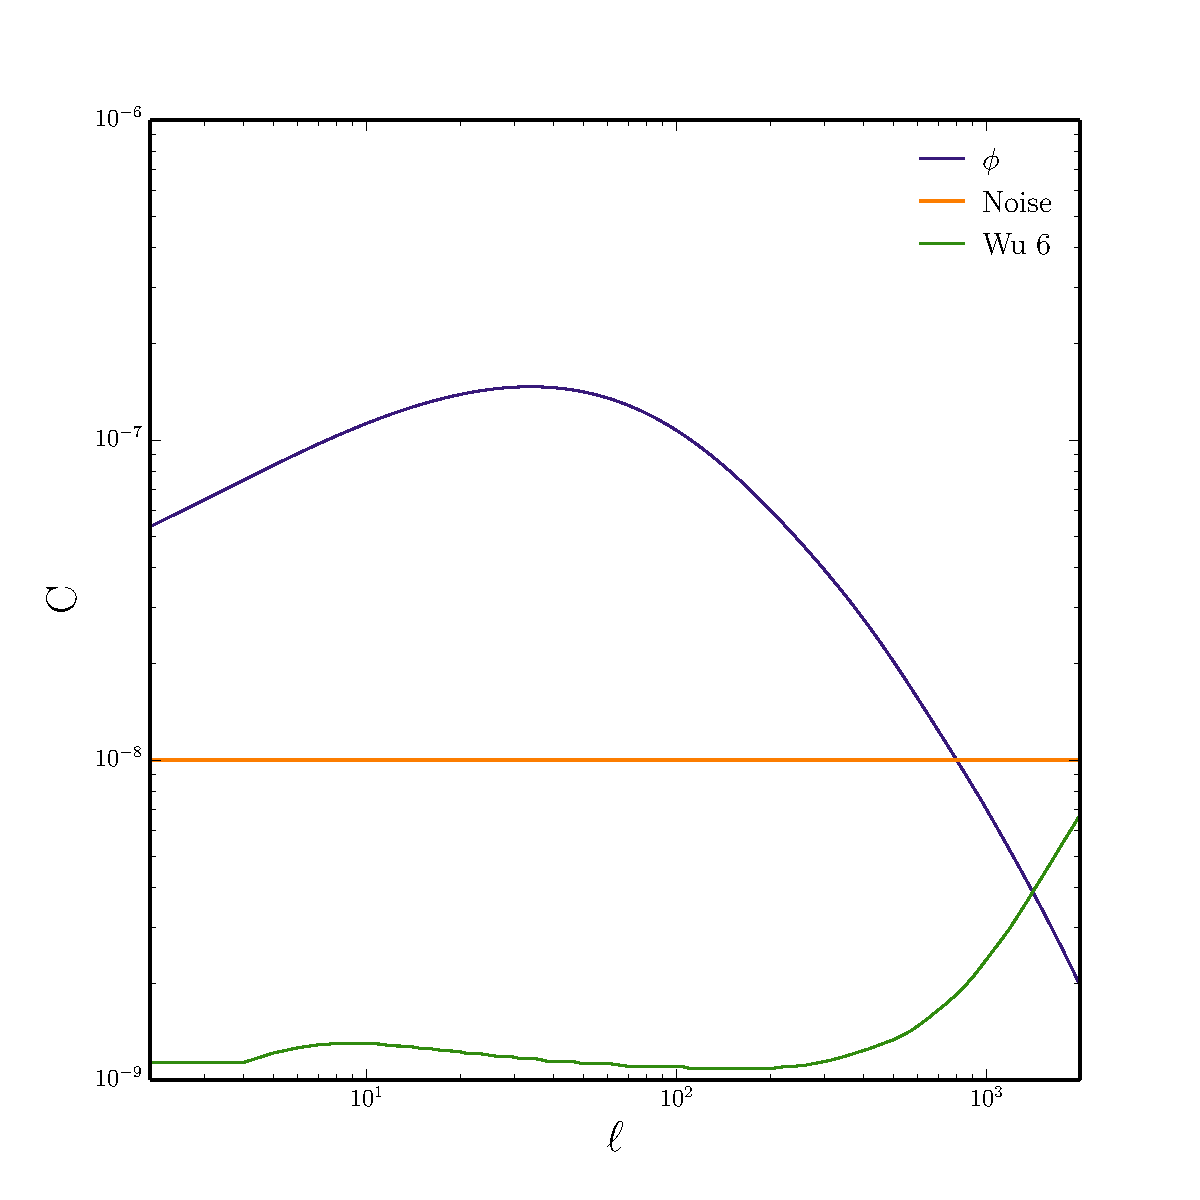
\includegraphics[scale=0.4]{PS_phi_with_noise.pdf}
\caption{Lensing potential power spectrum use in this work has a signal to noise bigger than one up to $\ell\simeq800-1000$.
In the figure: the deflection power spectrum for our fiducial cosmology together with the two examples of lensing reconstruction noise $N^{\phi}$ used in this work.}
\label{fig:phi-cl-noise}
\end{center}
\end{figure}

\begin{figure}[htbp]
\begin{center}
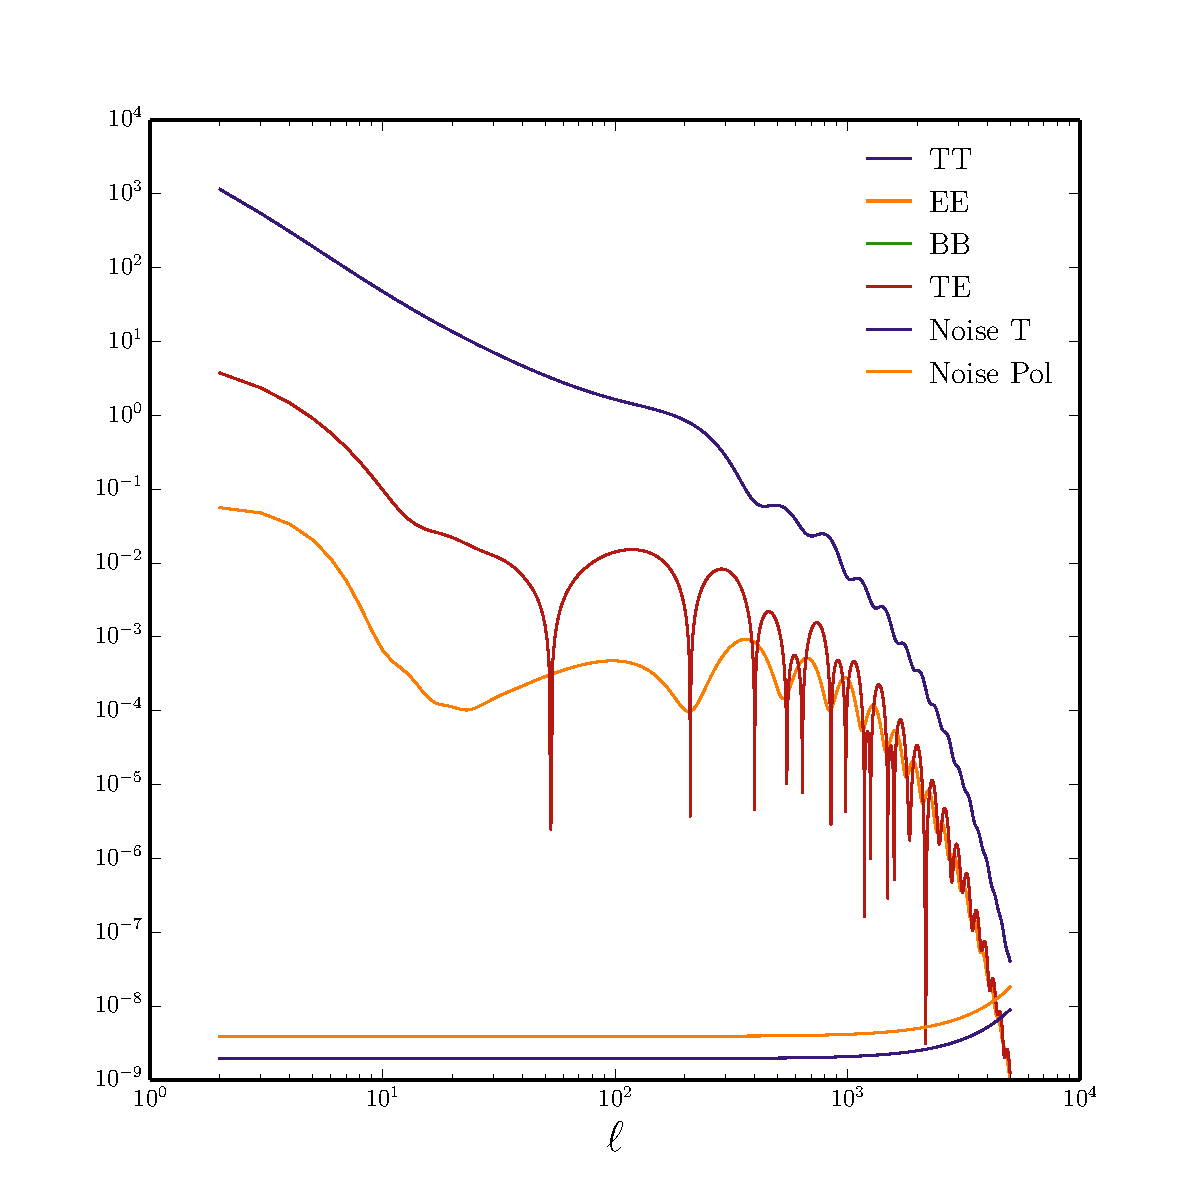
\includegraphics[scale=0.4]{PS_with_noise.pdf}
\caption{The next generation $C^{T,E}$ used in this work are almost cosmic variance limited.
In the figure: CMB power spectrum for our fiducial cosmology together with the instrumental noise used in this work.}
\label{fig:cmb-cl-noise}
\end{center}
\end{figure}


\subsection{CMB S4 experiments specifications.\label{subsec:cosmo-noise}}
In this subsection we describe the assumptions we made in calculating the elements that goes in \refeq{Fij_def2} and, in particular, the power spectra $C_{\ell}$ and the noise power $N_{\ell}$.
Firstly we parametrize our cosmology using a flat $\nu \Lambda$CDM universe. We allow a set different Dark Energy models by introducing the equations of state parameter $w$ as a varying parameter.
We chose our fiducial parameters following Table 2 of \textit{Planck} best fit \cite{planck-collaboration:2014g}, i.e. $\Omega_c h^2 = 0.12029$, $\Omega_b h^2 = 0.022068$, $A_s = 2.215\times10^{-9}$ at $k_0 = 0.05\ {\rm Mpc}^{-1}$, $n_s = 0.9624$, $\tau = 0.0925$, and $H_0 = 67.11$ km/s/Mpc. Regarding the $\Lambda$CDM extension, we chose a neutrino energy densities $\Omega_{\nu} h^2$=0.0009, which corresponds to $M_{\nu}$ $\simeq$ 85\ meV, a standard $N_{\rm eff}=3.046$ and a dark energy equation of state, $w=-1$.
Given the model, we use CAMB \cite{Lewis:1999bs} to compute the power spectra $C_{\ell}$ at the fiducial values and at those needed to compute derivatives using \refeq{deriv}. Notice that while we vary one parameter in \refeq{deriv} we keep all the others fixed with the exception of $\Omega_{\Lambda}$ which is always changed in order to keep the universe flat ($\Omega_{\rm k} = 0$).

The instrumental noise power $N_{\ell}^{T,E}$ and the lensing reconstruction $N_{\ell}^{\phi}$ in \refeq{Fij_def2} correspond to the expected level for the next generation of CMB experiments (S4).
For the temperature and E-mode polarization of the CMB, together with the improved depth and resolution we also assume that large scale foregrounds, like dust, are under control or negligible. We deal with the presence of point sources poisson noise in the temperature signal by simply discarding all the small scales modes with $\ell>\ell_{\rm T,max}=3000$.
The remaining source of noise, the instrumental noise, is added to the power spectrum in the usual way:
 \begin{equation}
 	\centering
		N^{X}_\ell = s^{\, 2} \exp \left(\ell(\ell+1) \frac{\theta^{\ 2}_{\textsc{fwhm}}}{8\log2}\right),
	\label{eq:beamnoise}
\end{equation}
where $\theta^{\ 2}_{\textsc{fwhm}}$ is the FWHM of the experiment's beam and $s$ represents the instrumental white noise.
We decide to use a level of noise $s = 1.5$ $\mu$K-arcmin for $X=T$ and a beam of $\theta_{\textsc{fwhm}}=1$ arcmin (PRELIMINARY).
Note that $1.5$ $\mu$K-arcmin is the noise in temperature and we need $s \rightarrow s\times \sqrt{2}$ in the case of polarization $ XX' = \{ EE, BB \}$.


Together with E and T we will use the information contained in the lensing potential $\phi$ as it is reconstructed from the CMB. The lensing potential represents the integration along the line of site of the gravitational potential and it leaves its signature in the CMB, both in temperature and polarization, by bending the trajectory of CMB photons. This introduces non gaussianities that couple different, otherwise independent, CMB modes and it can be reconstructed using a quadratic estimator technique \cite{okamoto:2003,hu:2002}.
For the noise $N_\ell^{\phi\phi}$ associated to the reconstructed $\phi$ we follow the non-iterative technique of \cite{okamoto:2003,hu:2002}.




%\begin{eqnarray}
%\centering
%	s\ [\;\mu {\rm K.arcmin}\;] \equiv \frac{ {\rm NET}\ [\; \mu{\rm K.}\sqrt{s}\;] \times \sqrt{f_{sky} \ [\;{\rm arcmin}^2\;] }}{ \sqrt {N_{\rm det} \times Y \times \Delta T\ [\;{\rm s }\;]}}.
%	\label{eq:sensitivity_definition}
%\end{eqnarray}
%



%\begin{eqnarray}
%	T_{\nu} = \left( \frac{4}{11} \right)^{1/3} T_{\gamma} 
%	\label{eq:tnu_propto_tgamma}
%\end{eqnarray}

\section{Results \label{sec:results}}
In this section we present our main results. We will start from 


{\bf Let's open up one parameter at a time: first standard LCDM with neff, and then with mnu, and then with w. Also, let's show a curve in each plot with constraints on *all*  parameters, not just one of them, as that will give people a sense of what is gained if multiple priors can be obtained.}

\subsection{Relativistic Degrees of Freedom, $N_{\rm eff}$}

In the standard cosmology, three active neutrinos are thermally produced in the early universe. Were they to decouple well before the epoch of electron-positron annihilation, their energy density after their decoupling would be equal to $3\times (7/8)\times (4/11)^{4/3}\,\rho_{\rm cmb}$, with the first factor capturing the contributions from the 3 active species; the second the difference between fermions and bosons; and the last the relative heating of the photons in the CMB by electron-positron annihilation. However decoupling is not a discrete event and occurs close to the time of electron-positron annihilation, so the neutrinos share a bit in the heating, with the factor of 3 replaced by $N_{\rm eff}=3.046$. The additional fraction depends not only on well-known neutrino scattering rates but also finite temperature quantum corrections. 
Upcoming experiment have the potential to measure this tiny deviation of $N_{\rm eff}$ from 3. This will be an amazing test of our understanding of the Universe when it was about a second old.
Furthermore any significant deviation from this value could be a hint of a different scenario not predicted by the standard model. 
%==========
\begin{figure}[htbp]
\begin{center}
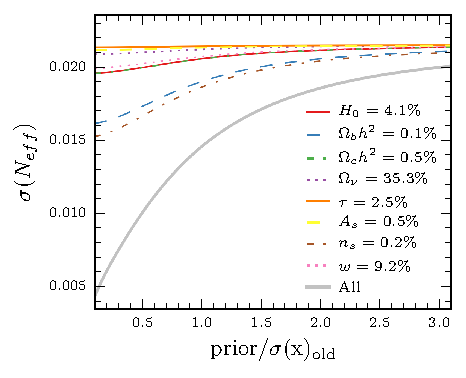
\includegraphics{prior_massless_neutrinos_snow_mass.pdf}
\caption{Projected 1-sigma error on $N_{\rm eff}$ as a function of the strength of the prior on the other 6 cosmological parameters of the standard $\Lambda$CDM model. Each prior is expressed in units of the error that would be obtained internally from our suite of CMB experiments; e.g., $\sigma(H_0)_{\rm old}=4.1\%$. The parameters that would be most useful to constrain externally for the purposes of determining $N_{\rm eff}$ are $n_s$ and $\Omega_bh^2$. The bottom-most (grey) curve shows the impact of imposing the given prior on {\it all} the other parameters simultaneously.}
\label{fig:prior_massless_neutrinos}
\end{center}
\end{figure}
%==========
\reffig{prior_massless_neutrinos} shows projections for how well our suite of CMB experiments will do at measuring $N_{\rm eff}$ as a function of priors on the other 6 parameters in the standard cosmological model ($H_0, \Omega_mh^2,\Omega_bh^2, n_s, A_s,$ and $\tau$). With no priors on the other parameters, the projected $1$-sigma error is  about $0.02$, suggesting a 2-sigma detection of the deviation from $N_{\rm eff}=3$. The sensitivity comes from the effect of extra species on the damping tail of the CMB anisotropies, both in temperature and polarization, so parameters that also affect the shape of the damping tail, like the slope $n_s$ and the baryon density $\Omega_bh^2$, are most degenerate with $N_{\rm eff}$. As such, \reffig{prior_massless_neutrinos} shows that obtaining external priors on either of these would reduce the errors on $N_{\rm eff}$ to ensure a 3-sigma detection of the partial decoupling prediction. The bottom-most curve shows that if all parameters were constrained externally, then the projected error on $N_{\rm eff}$ would improve significantly.


\subsection{Neutrino Masses}

Small scale structure formation is suppressed if fast-moving neutrinos comprise a significant part of the matter budget. This effect, probed by CMB lensing, will allow us to determine how much of the matter density is made up of neutrinos. Since the active neutrino number densities are known in the standard model, this can be directly transformed into a constraint on the the sum of the neutrino masses, $\sum m_\nu$. This is particularly exciting because there is a lower limit on $\sum m_\nu>0.05$ eV that emerges from oscillation experiments. 



\begin{figure}[htbp]
\begin{center}
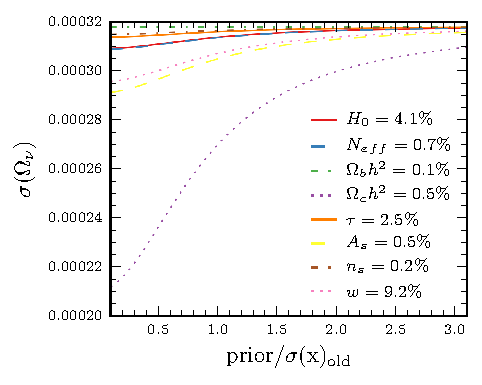
\includegraphics{prior_omnuh2_snow_mass.pdf}
\caption{Constraints on the sum of the neutrino masses as a function of priors on cosmological parameters, as in \reffig{prior_massless_neutrinos}.  Note that constraints would be improved significantly  by distance measurements that constrain $\Omega_ch^2$. The lower limit on the sum of the neutrino masses is 50 meV.}
\label{fig:prior_omeganuh2}
\end{center}
\end{figure}


\reffig{prior_omeganuh2} shows that, without any external priors, upcoming CMB experiments are poised to obtain 1-sigma limits on $\sum m_\nu$ of order 30 meV, corresponding to close to a 2-sigma detection even in the worst case scenario. Adding in external priors helps this significantly though, as discussed in \citet{2013arXiv1309.5383A}. There, the prior was deescribed as ``DESI BAO'', that is a measurement of distances as a function of redshift from the baryon acoustic oscillation feature probed by DESI. Here, the same improvement is parametrized by a strong prior on $\Omega_ch^2$, which indeed determines these low-redshift distances. As found in \cite{2013arXiv1309.5383A}, the projected error falls below 20 meV with this prior. Adding in other priors would help further.

%\begin{table}[htdp]
%\begin{center}
%\begin{tabular}{|c|c|}
%\hline
%$H_{0}$ & $67.11$ km/s/Mpc\\
%\hline
%\hline
%$\tau$ & $0.0925$ \\
%\hline
%
%\hline
%$A_{s}$ &$2.215 \times 10^{-9}$ \\
%\hline
%
%\hline
%$n_{s}$ & $0.9624$ \\
%\hline
%
%\hline
%$N_{eff}$ & 3.046\\
%\hline
%\end{tabular}
%\end{center}
%\caption{Fiducial values of cosmological parameters used in this work.}
%\label{default}
%\end{table}%

\subsection{Dark Energy Equation of State}

While the primordial CMB has limited information about the late-time dark energy equation of state, CMB lensing probes the growth of structure at late times and therefore is sensitive to $w$. Here we are using only the information from the lensing power spectrum as inferred from the CMB, but there is even more information not considered here contained in the many galaxy clusters that upcoming missions will detect via the Sunyaev-Zel'dovich effect. 


\begin{figure}[htbp]
\begin{center}
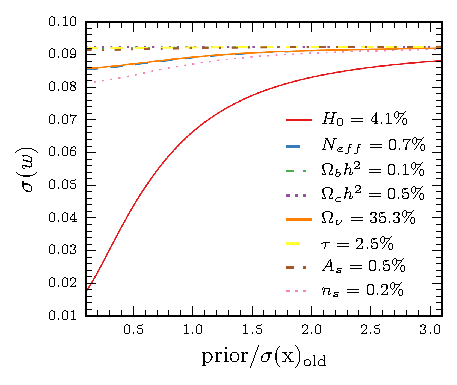
\includegraphics{prior_w_snow_mass.pdf}
\caption{Constraints on the dark energy equation of state $w$ as a function of priors on cosmological parameters, as in \reffig{prior_massless_neutrinos}. An external prior on $H_{0}$ will be crucial to improve the constraint.} 
\label{fig:prior_w}
\end{center}
\end{figure}

\reffig{prior_w} shows that without any priors, CMB experiments will not do much better than current constraints, which hover around 10\%. However, an external constraint on the Hubble constant would improve the CMB constraints on $w$ considerably. {\bf We should try to understand why.}


%{\bf I don't really understand this table.}
%\begin{table}[htdp]
%
%\begin{center}
%\begin{tabular}{|c|c|c|c|c|c|c|}
%\hline
%$H_{0}$ &$ M_{\nu}$ &$\Omega_{bc}h^{2}$&$\Omega_{b}h^{2}$&$\tau$&$A_{s}$&$n_{s}$ \\
%$0.80 \%$&$40.92\%$&$0.44\%$&$0.11\%$&$3.075\%$&$0.53\%$&$0.18\%$\\
%
%\hline
%\end{tabular}
%\caption{How well we do constrain separate parameters with this data without any external prior? Things to notice: this is done with the Zhen test parameters ($\ell<3000$ and no error on lensing). Now if we trust it CMB alone can get a $0.8\%$ error on $H_{0}$ thus I am not surprised if a prior on H would not help. However what do we think about it? is it really CMB better than SN. People will not agree on that. $\tau$ will probably improve and also M$\nu$ from BAO may help improving parameters.}
%\end{center}
%\label{default}
%\end{table}%



% tables should appear as floats within the text
%
% Here is an example of the general form of a table:
% Fill in the caption in the braces of the \caption{} command. Put the label
% that you will use with \ref{} command in the braces of the \label{} command.
% Insert the column specifiers (l, r, c, d, etc.) in the empty braces of the
% \begin{tabular}{} command.
% The ruledtabular enviroment adds doubled rules to table and sets a
% reasonable default table settings.
% Use the table* environment to get a full-width table in two-column
% Add \usepackage{longtable} and the longtable (or longtable*}
% environment for nicely formatted long tables. Or use the the [H]
% placement option to break a long table (with less control than 
% in longtable).
% \begin{table}%[H] add [H] placement to break table across pages
% \caption{\label{}}
% \begin{ruledtabular}
% \begin{tabular}{}
% Lines of table here ending with \\
% \end{tabular}
% \end{ruledtabular}
% \end{table}

% Surround table environment with turnpage environment for landscape
% table
% \begin{turnpage}
% \begin{table}
% \caption{\label{}}
% \begin{ruledtabular}
% \begin{tabular}{}
% \end{tabular}
% \end{ruledtabular}
% \end{table}
% \end{turnpage}

% Specify following sections are appendices. Use \appendix* if there
% only one appendix.

%\appendix
%\section{Marginalization , not needed probably}
%\begin{equation}
%G = F^{\phi\phi} - F^{\phi\psi}U\Lambda^{-1}U^{T}F^{\phi\psi},
%\end{equation}
%where we define $\phi = \{N_{eff},...\}$ and $\psi = \{\Omega_{m} ... marginal\}$; therefore, $F^{\phi\phi}$ is the block of the total Fisher matrix containing the parameters we want to constrain, whilst $F^{\psi\psi}$ is the nuisance-parameter Fisher sub-matrix. Here, $\Lambda$ is the diagonal matrix whose elements are the eigenvalues of $F^{\psi\psi}$, whilst U is the orthogonal matrix diagonalising $F^{\psi\psi}$. By using Eq., our marginalizing procedure is more stable, since degeneracies in $F^{\phi\phi}$ are properly propagated to G with no instabilities, and we do not even worry about a possibly ill-conditioned $F^{\phi\phi}$ sub-matrix, since we check its stability on the fly by the diagonalisation.

\begin{acknowledgments}
We thank Youngsoo Park for his contribution in the early stage of this work.
AM wants to thank Zhen Pan who allows a careful cross-check of our results.
This work was partially supported by the Kavli Institute for Cosmological Physics at the University of Chicago through grants NSF PHY-1125897 and an endowment from the Kavli Foundation and its founder Fred Kavli.
%%%=================================================================
The work of SD is supported by the U.S. Department of Energy, including grant DE-FG02-95ER40896.
\end{acknowledgments}

% Create the reference section using BibTeX:
\bibliography{N_eff_prior_paper}

\end{document}


